%\documentclass[
  bibliography=totoc,     % Literatur im Inhaltsverzeichnis
  captions=tableheading,  % Tabellenüberschriften
  titlepage=firstiscover, % Titelseite ist Deckblatt
]{scrartcl}

% Paket float verbessern
\usepackage{scrhack}

% Warnung, falls nochmal kompiliert werden muss
\usepackage[aux]{rerunfilecheck}

% unverzichtbare Mathe-Befehle
\usepackage{amsmath}
% viele Mathe-Symbole
\usepackage{amssymb}
% Erweiterungen für amsmath
\usepackage{mathtools}

% Fonteinstellungen
\usepackage{fontspec}
% Latin Modern Fonts werden automatisch geladen
% Alternativ zum Beispiel:
%\setromanfont{Libertinus Serif}
%\setsansfont{Libertinus Sans}
%\setmonofont{Libertinus Mono}

% Wenn man andere Schriftarten gesetzt hat,
% sollte man das Seiten-Layout neu berechnen lassen
\recalctypearea{}

% deutsche Spracheinstellungen
\usepackage[ngerman]{babel}


\usepackage[
  math-style=ISO,    % ┐
  bold-style=ISO,    % │
  sans-style=italic, % │ ISO-Standard folgen
  nabla=upright,     % │
  partial=upright,   % │
  mathrm=sym,        % ┘
  warnings-off={           % ┐
    mathtools-colon,       % │ unnötige Warnungen ausschalten
    mathtools-overbracket, % │
  },                       % ┘
]{unicode-math}

% traditionelle Fonts für Mathematik
\setmathfont{Latin Modern Math}
% Alternativ zum Beispiel:
%\setmathfont{Libertinus Math}

\setmathfont{XITS Math}[range={scr, bfscr}]
\setmathfont{XITS Math}[range={cal, bfcal}, StylisticSet=1]

% Zahlen und Einheiten
\usepackage[
  locale=DE,                   % deutsche Einstellungen
  separate-uncertainty=true,   % immer Unsicherheit mit \pm
  per-mode=symbol-or-fraction, % / in inline math, fraction in display math
]{siunitx}

% chemische Formeln
\usepackage[
  version=4,
  math-greek=default, % ┐ mit unicode-math zusammenarbeiten
  text-greek=default, % ┘
]{mhchem}

% richtige Anführungszeichen
\usepackage[autostyle]{csquotes}

% schöne Brüche im Text
\usepackage{xfrac}

% Standardplatzierung für Floats einstellen
\usepackage{float}
\floatplacement{figure}{htbp}
\floatplacement{table}{htbp}

% Floats innerhalb einer Section halten
\usepackage[
  section, % Floats innerhalb der Section halten
  below,   % unterhalb der Section aber auf der selben Seite ist ok
]{placeins}

% Seite drehen für breite Tabellen: landscape Umgebung
\usepackage{pdflscape}

% Captions schöner machen.
\usepackage[
  labelfont=bf,        % Tabelle x: Abbildung y: ist jetzt fett
  font=small,          % Schrift etwas kleiner als Dokument
  width=0.9\textwidth, % maximale Breite einer Caption schmaler
]{caption}
% subfigure, subtable, subref
\usepackage{subcaption}

% Grafiken können eingebunden werden
\usepackage{graphicx}

% schöne Tabellen
\usepackage{tabularray}
\UseTblrLibrary{booktabs, siunitx}

% Verbesserungen am Schriftbild
\usepackage{microtype}

% Literaturverzeichnis
\usepackage[
  backend=biber,
]{biblatex}
% Quellendatenbank
\addbibresource{lit.bib}
\addbibresource{programme.bib}

% Hyperlinks im Dokument
\usepackage[
  german,
  unicode,        % Unicode in PDF-Attributen erlauben
  pdfusetitle,    % Titel, Autoren und Datum als PDF-Attribute
  pdfcreator={},  % ┐ PDF-Attribute säubern
  pdfproducer={}, % ┘
]{hyperref}
% erweiterte Bookmarks im PDF
\usepackage{bookmark}

% Trennung von Wörtern mit Strichen
\usepackage[shortcuts]{extdash}

\author{%
  Vincent Wirsdörfer\\%
  \href{mailto:vincent.wirsdoerfer@udo.edu}{authorA@udo.edu}%
  \and%
  Joris Daus\\%
  \href{mailto:joris.daus@udo.edu}{authorB@udo.edu}%
}
\publishers{TU Dortmund – Fakultät Physik}


%\begin{document}

\section{Versuchsdurchführung}
\label{sec:Versuchsdurchfuehrung}

Zu Beginn des Versuchs werden die Eigenschaften der vorliegenden Materialen untersucht. Konkret bedeutet dies,
dass die Länge und Gewichte der Probestäbe gemessen werden. Zusätzlich werden die bereits beschrifteten Gewichte gewogen,
um signifikante, grundsätzliche Fehler ausschließen zu können. Im Folgenden wird sich genauer mit den einzelnen Elementen
und der Funktionsweise der Versuchsapperatur vertraut gemacht.

\begin{figure}[H]
    \centering
    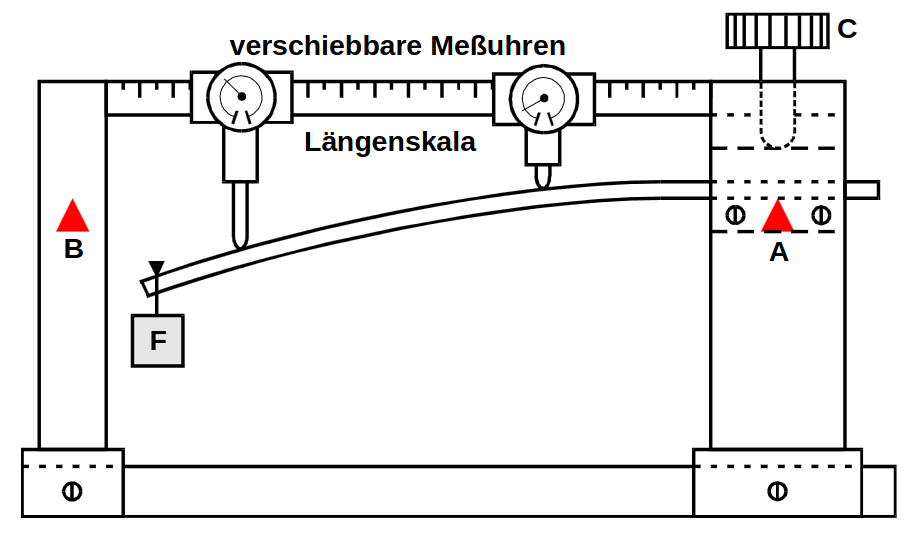
\includegraphics[height=5cm]{./content/Versuchsaufbau.png}
    \caption{Beschreibung der Versuchsapperatur.}
    \label{fig:Versuchsaufbau}
\end{figure}

\subsection{Einseitige Einspannung}
\label{sec:Einseitig}
Gemäß Abbildung \ref{fig:Versuchsaufbau} werden die Stäbe bei der einseitigen Einspannung auf dem Fußpunkt A gelagert
und durch die Spannvorrichtung C fest montiert. Nun wird die effektive Länge des Stabes $L$ gemessen, also der Abstand vom Ende des Stabes bis zur Einspannung.
Im Anschluss wird eine sinnvolle Intervallschachtelung gewählt, sodass mit etwa 15-20 Messungen ein Großteil der Länge des Stabes
durch Messungen abgedeckt wird. Die in der Abbildung \ref{fig:Versuchsaufbau} dargestellte Kraft $F$ erfolgt durch Anhängen eines
Gewichts der Masse $m = 0.5\,\unit{\kilo\gram}$. Hierbei werden die Messuhren nach jeder einzelnen Messung erneut geeicht und
die Messdaten in ein Heft eingetragen.

\subsection{Beidseitige Einspannung}

Auf der linken Seite Abbildung \ref{fig:Versuchsaufbau} ist ein weiterer Fußpunkt B zu erkennen. Auf Diesem wird nun das
andere Ende der Stäbe angeleget und befestigt. Durch die beiden Fußpunkte sind die Stäbe nun beidseitig in der Apperatur
eingespannt. Nun wird der Abstand zwischen den maximalen Auslenkungen der Messuhren gemessen. Das Gewicht soll somit in der
Mitte dieses Abstandes aufgehangen werden und besitzt nun eine Masse von $m = 1\,\unit{\kilo\gram}$. Durch die simultane Messung der linken und rechten Seite verkürzt sich die jeweils
zu messende Strecke im Vergleich zur vorherigen Methode \ref{sec:Einseitig}, weswegen nur 10-15 Messungen pro Seite 
aufgenommen werden. Analog zur einseitigen Einspannung werden die Messuhren nach jeder Messung auf Null geeicht und die Messdaten notiert.

%\end{document}

